% Correcting the title chapter page
\fancypagestyle{plain}{%
    \fancyhf{}
    \fancyhead[RO,LE]{\bfseries \thepage}
    \fancyhead[CO]{\rightmark}
    \fancyhead[CE]{\leftmark}
    \renewcommand{\headrulewidth}{0.4pt}}

\chapter{Simetrije u klasičnoj i kvantnoj mehanici}
\label{ch:klasicna}

\section{Transformacije i tenzori}

\begin{definicija}
Fizikalna veličina je \emph{invarijantna} na neku transformaciju ako se
pri toj transformaciji ne mijenja.

Jednadžba koja opisuje fizikalni sustav je \emph{kovarijantna}
na neku transformaciju ako se pri toj transformaciji 
njen \emph{oblik} ne mijenja.
\end{definicija}

Primjer: masa i naboj su invarijantne na rotacije.

Primjer: Newtonove jednadžbe za sustav dva tijela koja gravitiraju
\begin{eqnarray}
 m_1 \ddot{\vec{r}}_1 & = & G \frac{m_1 m_2}{|\vec{r}_2 - \vec{r}_1|^3}
    (\vec{r}_2 - \vec{r}_1) \label{eq:newton1} \\
 m_2 \ddot{\vec{r}}_2 & = & G \frac{m_1 m_2}{|\vec{r}_1 - \vec{r}_2|^3}
    (\vec{r}_1 - \vec{r}_2)
\end{eqnarray}
su kovarijantne pri rotacijama. Uvjerimo se u to.
Rotiramo za neki kut:
\begin{align*}
(\vec{r}_{1})_i \to (\vec{r}_{1}')_i &= \sum_j R_{ij}(\hat{\vec{n}},\theta) 
   (\vec{r}_{1})_j \;, \qquad& \text{(po komponentama)}\\
\text{tj.}\qquad \vec{r}_{1}\to \vec{r}_{1}' &= R(\hat{\vec{n}},\theta) 
   \vec{r}_{1}\;, \qquad& \text{(matrično)}
\end{align*}
i isto za $\vec{r}_2$.

Ovdje je $R(\hat{\vec{n}},\theta)$ standardna matrica rotacije u trodimenzionalnom
prostoru, npr. za rotaciju oko $z$-osi
\begin{equation}
R(\hat{\vec{z}},\theta) = \begin{pmatrix}
\cos\theta &  -\sin\theta &  0 \\
\sin\theta &  \cos\theta &  0 \\
    0  &       0     &  1 
\end{pmatrix} \;.
\label{eq:matrot}
\end{equation}

Sada iz (\ref{eq:newton1}) slijedi da je u transformiranim koordinatama
jednadžba za npr. $\vec{r}'_1$ 
\begin{equation*}
\begin{split}
m_1 \ddot{\vec{r}}'_1 &= m_1 R \ddot{\vec{r}}_1 \\
   &= G \frac{m_1 m_2}{|\vec{r}_2 - \vec{r}_1|^3}
    (R\vec{r}_2 - R\vec{r}_1) \\
   &= G \frac{m_1 m_2}{|\vec{r}_2 - \vec{r}_1|^3}
    (\vec{r}'_2 - \vec{r}'_1) \\
   &= G \frac{m_1 m_2}{|\vec{r}'_2 - \vec{r}'_1|^3}
    (\vec{r}'_2 - \vec{r}'_1) \;,
\end{split}
\end{equation*}
i isto za $\vec{r}'_2$, gdje smo radi jednostavnosti prestali
pisati argumente matrice rotacije $R = R(\vec{n},\theta)$.
Dakle, jednadžbe zarotiranog sustava imaju isti oblik
(kovarijantne su) premda su konkrentne vektorske veličine
u njima različite tj. $\vec{r}'_{1,2} \neq \vec{r}_{1,2}$.

Ova i daljnja diskusija podrazumijevaju da govorimo o \emph{aktivnim}
transformacijama koje djeluju na sam fizikalni sustav. U \emph{pasivnom}
pristupu u kojem transformiramo samo koordinatni sustav
ovako napisane jednadžbe su \emph{invarijantne} jer
ako $\vec{r}$ i $\vec{F}$ promatramo kao elemente vektorskog prostora,
a ne kao trojke koordinata tih vektora u nekoj bazi, onda rotacija
koordinatnog sustava ne mijenja same vektore i ono sto je onda
\emph{kovarijantno} je zapis tih jednadžbi po komponentama:
        
\begin{displaymath}
       m  \ddot{x}_{i} =  F_{i} \;.
\end{displaymath}


Kako prepoznajemo kovarijantne jednadžbe?

\begin{eqnarray*}
 \nabla\times\vec{B}=\vec{J}+\frac{\partial \vec{E}}{\partial t}
    &\textrm{ima oblik}&  \textrm{vektor=vektor + vektor} \\
 \nabla\cdot\vec{E}=\rho
    &\textrm{ima oblik}&  \textrm{skalar=skalar} \\
\end{eqnarray*}

 Što je skalar? Što je vektor?

Za razmatranje kovarijantnosti jednadžbi pri rotacijama određujuće svojstvo 
vektora nije to što je on opisan trojkom brojeva ili 
to što je on element nekog vektorskog prostora već je ključno na koji
se način on transformira pri rotacijama:

\vspace*{2ex}
\centerline{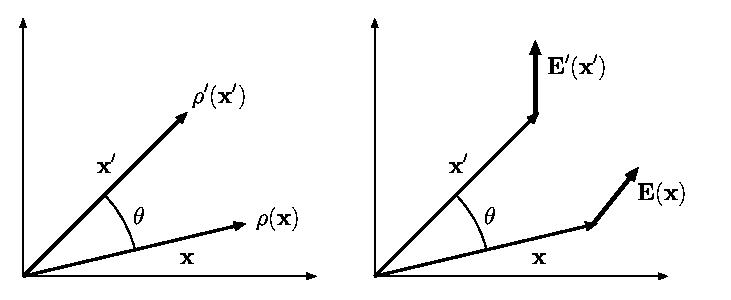
\includegraphics[scale=0.8]{pics/skalarvektor.eps}}

\begin{eqnarray*}
 \rho(\vec{r}) \to \rho'(\vec{r}') = \rho(\vec{r}) & : & \textrm{skalar} \\
  E_i(\vec{r}) \to E'_i(\vec{r}') = \sum_j R_{ij}E_j(\vec{r})
   & : & \textrm{vektor} \;,
\end{eqnarray*}
gdje je $R_{ij}$ ista matrica (poput (\ref{eq:matrot})) koja rotira
vektor položaja $\vec{r}$.

  Ovo se poopćuje na veličine sa složenijim transformacijskim svojstima,
\emph{tenzore}. 

\begin{definicija}
\label{def:tenzor}

\emph{Tenzor $n$-tog ranga} (pri rotacijama)  jest veličina $\bbtensor{T}$  koja
se transformira kao

\begin{displaymath}
 \bbtensor{T}_{i_1 i_2 \ldots i_n}(\vec{r}) \to \bbtensor{T}'_{i_1 i_2 \ldots i_n}(\vec{r}') =
\sum_{j_1, j_2, \ldots, j_n}
  R_{i_1 j_1}  R_{i_2 j_2} \ldots  R_{i_n j_n} \bbtensor{T}_{j_1 j_2 \ldots j_n}(\vec{r})
 \; . 
\end{displaymath}
\end{definicija}


Primjeri:
\begin{itemize}
\item skalari su tenzori nultog ranga
\item vektori su tenzori prvog ranga.
\item Ohmov zakon u neizotropnom sredstvu (npr. kristalu): 
\begin{equation*}
j_i = \sum_j \sigma_{ij} E_j
\end{equation*}
$\sigma_{ij}$ --- tenzor električne vodljivosti (tenzor drugog ranga)

\item $F_{\mu\nu}$ --- tenzor elektromagnetskog polja (tenzor drugog
ranga, ali obzirom na Lorentzove transformacije)

\item Zakrivljenost $n$-dimenzionalnih ploha se standardno opisuje
tzv. Riemannovim tenzorom $R_{abcd}$  (tenzor četvrtog ranga)
\end{itemize}



 Komponente tenzora drugog ranga možemo prikazati matricom.

 Tenzorsko svojstvo je vezano uz tip transformacije. Tako postoje
npr. Lorentzovi vektori (četvero-vektori), izovektori, itd.  Kad se tip
transformacije ne specificira misli se na rotacije (gornji
vektori su vektori obzirom na rotacije). 

 Da bi jednadžba bila kovarijantna svi njeni članovi se moraju transformirati
na isti način. (Kažemo: moraju se transformirati kovarijantno.)
To znači da moraju pripadati istoj reprezentaciji grupe transformacija.
("Pripadati" u smislu da na svakog djeluje ista reprezentacija. Nisu oni
sami reprezentacije!)


\emph{Napomena:}  Pojmovi kovarijantnosti i kontravarijantnosti
komponenata vektora i tenzora koje srećemo u teoriji relativnosti
(``gornji'' i ``donji'' indeksi, vidi slijedeći odjeljak), a 
zapravo potječu iz diferencijalne 
geometrije nemaju veze s ovom kovarijantnosti.  To su samo homonimi.
 
 Kakve su posljedice kovarijantnosti jednadžbi gibanja na njihova
rješenja?

  Pojedina rješenja sama za sebe naravno nisu invarijantna, ali 
kovarijantnost jednadžbi gibanja implicira da transformacijom rješenja
dobijemo također dobro rješenje.

Primjer: dva gravitirajuća tijela s reduciranom koordinatom $\vec{r}
= \vec{r}_1 - \vec{r}_2$. 
Rješenje jednadžbi gibanja je funkcija $\vec{r}(t)$ --- elipsa u prostoru.
Međutim, translatirana elipsa $\vec{r}_{1,2}(t)+\vec{a}$ i zarotirana
elipsa $R\vec{r}_{1,2}(t)$ su isto dobra rješenja za svaki $\vec{a}$ i $R$
u što se lako uvjerimo uvrštavanjem u Newtonove jednadžbe.

To da translacijom (rotacijom) rješenja također dobijemo rješenje je posljedica
homogenosti (izotropije) prostora.

Provedemo li unatrag ovaj logički sljed vidimo da homogenost
(izotropija) prostora zahtjeva da jednadžbe gibanja budu kovarijantne
obzirom na translacije (rotacije).


Protuprimjer: vremenska inverzija (diskretna grupa = $Z_2$) \\
  S jedne strane gornje Newtonove jednadžbe su kovarijantne i obzirom na vremensku
inverziju. I stvarno, vremenski invertirano rješenje dvaju gravitirajućih
tijela u gibanju je također dobro rješenje tj. mogući slučaj u prirodi.
No, vremenska inverzija plina koji slobodno izlazi iz plinske boce nije
moguć događaj što ukazuje na to da priroda nije simetrična na vremensku inverziju i
jednadžbe koje opisuju ekspanziju plina ne bi smjele biti kovarijantne
na takvu inverziju. Koje su to jednadžbe? ($\to$Problem strijele vremena.)


% \subsection*{Očuvanje veličina i simetrije}
% 
%  Lagrange-Hamiltonova formulacija klasične mehanike je pogodnija od
% Newtonove za formalizaciju principa simetrije.
% 
% \begin{description}
% \item[a)] prostorne translacije \\
%   \begin{displaymath}
%   \vec{r}\to\vec{r}'=\vec{r}+\delta\vec{r} \qquad \textrm{grupa} 
%            (\mathbb{R}^{3},+)
%  \end{displaymath}
% \begin{displaymath}
%  \delta L = L(\vec{r}', \dot{\vec{r}}', t) -  L(\vec{r}, \dot{\vec{r}}, t)
%  =0
% \end{displaymath}
% \begin{displaymath}
%  \delta L = \frac{\pd L}{\pd r_i} \delta r_i =0
% \imp \frac{\pd L}{\pd r_i}=0 \quad i=1,2,3 \;,
% \end{displaymath}
% jer \emph{homogenost prostora} traži da promjena lagranžijana bude nula
% za proizvoljan pomak $\delta r_i$.  Kao posljedica toga, lagranžijan
% $L(\vec{r},\dot{\vec{r}},t)=L(\dot{\vec{r}},t)$ ne ovisi eksplicitno
% o koordinati $\vec{r}$.
% 
% Sada Euler-Lagrangeove jednadžbe,
% \begin{displaymath}
%   \frac{\pd L}{\pd r_i}-\frac{d}{d t} \frac{\pd L}{\pd \dot{r}_i}=0
% \end{displaymath}
% daju zakon očuvanja impulsa:
% \begin{displaymath}
% \frac{d}{d t} \frac{\pd L}{\pd \dot{r}_i}=
% \frac{d}{d t} p_i =0  \imp \vec{p}=\textrm{const.} \;.
% \end{displaymath}
% 
% \secret{Razjasniti što je s ZSI u sustavu dva tijela. Naizgled lagranžijan
% je funkcija od $r$, jer je $V\propto 1/r$.}
% 
% \item[b)] vremenske translacije
%  \begin{displaymath}
%   t \to t'=t+\delta t \qquad \textrm{grupa} (\mathbb{R},+)
% \end{displaymath}
% \begin{displaymath}
%  \frac{d L}{d t}=0
% \end{displaymath}
% Lagranžijan $L(\vec{r},\dot{\vec{r}},t)=L(\vec{r},\dot{\vec{r}})$ ne
% ovisi eksplicitno o vremenu $\to$ \emph {homogenost vremena}
% \begin{displaymath}
%  \frac{d L}{d t}=\frac{\pd L}{\pd r_i} \frac{\pd r_q}{\pd t} +
%                  \frac{\pd L}{\pd \dot{r}_i} \frac{\pd \dot{r}_i}{\pd t}
% =\frac{d}{d t}\left(\frac{\pd L}{pd \dot{r}_i}\dot{r}_i \right)
% =\frac{d}{d t}(p_i \dot{r}_i)
% \end{displaymath}
% \begin{displaymath}
%  \imp \frac{d}{d t} (p_i \dot{r}_i - L)=\frac{d}{d t} H =0
%  \imp E = \textrm{const}
% \end{displaymath}
% 
%   Energija je očuvana i to ne samo za izolirane sustave već i za sustave
% u konstantnom vanjskom polju.
% 
%  G(t) $\imp$ perpetuum mobile \secret{(http://www.emmynoether.com)}
% 
% \item[c)] prostorne rotacije \\
%   \begin{displaymath}
%   \vec{r}\to\vec{r}'=\vec{r}+\delta\phi\, \unitn\times\vec{r} 
% \qquad \text{grupa SO(3)}
%  \end{displaymath}
% \centerline{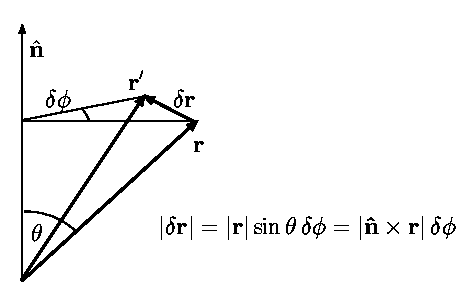
\includegraphics[scale=0.8]{pics/infrotacija.eps}}
% \begin{displaymath}
%  \delta L = \frac{\pd L}{\pd r_i}\delta{r_i} +
%             \frac{\pd L}{\pd \dot{r}_i}\delta{\dot{r}_i}
% = \dot{p}_i \delta\phi(\unitn\times\vec{r})_i +
%         p_i \delta\phi(\unitn\times\dot{\vec{r}})_i
% \end{displaymath}
% što zahvaljujući svojstvu cikličnosti miješanog vektorskog produkta
% prelazi u 
% \begin{displaymath}
% \delta L = \delta\phi \hat{n}_i (\vec{r}\times\dot{\vec{p}}+
%   \dot{\vec{r}}\times\vec{p})_i
% =\delta\phi \hat{n}_i \frac{d}{d t} (\vec{r}\times\vec{p})_i=0
% \end{displaymath}
% \emph{Izotropija prostora} znači da je varijacija lagranžijana
% neovisna o smjeru $\unitn$ pa je
% \begin{displaymath}
%   \vec{L}=\vec{r}\times\vec{p}=\textrm{const}
% \end{displaymath}
% \end{description}
% 
% 
% \textbf{Noetherin teorem}: Ako je sustav invarijantan na $n$-parametarsku
% grupu transformacija onda postoji $n$ konstanti gibanja.
% 

\section{Tenzori kao matematički strojevi$^{*}$}

Tenzore možemo promatrati kao neku vrstu \emph{matematičkih strojeva}
čiji ``input'' su jedan ili više vektora, a ``output'' vektor ili
skalar. 

Praktično, problemi kojima se bavimo se gotovo uvijek daju formulirati
u obliku ``\emph{Znamo te i te vektore koji opisuju sustav. Koliki
je $s$ ili $\vec{v}$ tog sustava?}'', gdje su $s$ i $\vec{v}$ neki
zanimljivi skalari ili vektori (energija, impuls, položaj, \dots).

Označimo tip tenzora $\bbtensor{T}$ s uređenim parom $(0, n)$ ukoliko 
$\bbtensor{T}$ predstavlja stroj čiji input je $n$ vektora, a output skalar,
a s $(1, n)$ ukoliko je output vektor. Takav stroj
možemo skicirati kao
\begin{equation}
   \bbtensor{T}(\underbrace{\slot, \slot, \slot, \dots}_{n \times})  \;,
\end{equation}

gdje su ``$\rule{1em}{1pt}$'' mjesta gdje treba staviti konkretne vektore
koje će onda stroj ``preraditi'' u rezultirajući skalar ili vektor

\begin{equation}
   \bbtensor{T}(\vec{v}_1, \vec{v}_2, \dots) = s \quad \text{ili} \quad \vec{v} \;.
\end{equation}

Na primjer, klasični vektor \emph{sile} možemo interpretirati kao
$(0, 1)$ tenzor $\bbtensor{SILA}(\slot)$ sa svojstvom da kad mu
u njegov slot stavimo vektor brzine dobijemo skalar snage:
\begin{equation}
   \bbtensor{SILA}(\vec{v}) = P
\end{equation}
gdje je unutranji ``mehanizam'' stroja dan jednadžbom $P = \vec{F}\cdot\vec{v}$.

Primjer $(0,2)$ tenzora je metrički tenzor $\bbtensor{G}(\slot, \slot)$,
čiji je mehanizam takav da kad u njegove slotove stavimo dva vektora
dobijemo njihov skalarni produkt:

\begin{equation}
   \bbtensor{G}(\vec{a}, \vec{b}) = \vec{a}\cdot\vec{b} \;.
\end{equation}

Ono što se često naziva tenzorom drugog ranga (matrica brojeva) su
samo komponente tenzora u nekoj bazi, koje se
dobiju kad se pravom apstraktnom tenzoru u njegove input slotove
stave jedinični bazni vektori, npr,

\begin{equation}
   \bbtensor{G}(\vec{e}_i, \vec{e}_j) = g_{ij} \;.
\label{eq:Gkomponente}
\end{equation}

Tenzor gustoće vodljivosti iz prošlog odjeljka je dakle
tipa $(1,1)$, odnosno $\sigma(\slot)$, jer imamo
$\sigma(\vec{E}) = \vec{j}$, dakle jedan vektor kao input
i drugi kao output.

Totalno antisimetrični tenzor (Levi-Civita) u tri dimenzije je
tenzor oblika $(1, 2)$, u svom obliku u kojem nam daje
vektorski produkt dvaju vektora
\begin{equation}
   \bbtensor{LEVICIVITA}(\vec{a}, \vec{b}) = \vec{a}\times\vec{b} \;,
\end{equation}
ali on može biti u obliku $(0, 3)$ kad daje mješani produkt 
triju vektora
\begin{equation}
   \bbtensor{LEVICIVITA}'(\vec{a}, \vec{b}, \vec{c}) =
 (\vec{a}\times\vec{b})\cdot\vec{c} \;,
\end{equation}
gdje ta dva oblika nisu identična.

U elektrodinamici (koja je teorija koja poštuje specijalnu teoriju
relativnosti), javlja se $(1,1)$ tenzor $\bbtensor{FARADAY}$, ali koji
nije tenzor obzirom na rotacije
već obzirom na relativističke transformacije u četverodimenzionalnom
prostoru Minkowskog. Taj tenzor daje četverovektor Lorentzove sile
kad mu se kao input stavi četverovektor brzine
$\bbtensor{FARADAY}(\vec{u)} = F_{\rm Lorentz}$, odnosno u uobičajenom
zapisu po komponentama $\mu, \nu = 0,1,2,3$, 
$F^{\mu}_{\rm Lorentz} = d p^{\mu}/d\tau = e F^{\mu}_{\,\nu} u^\nu$.

\secret{
Riemannov tenzor zakrivljenosti plohe spomenut u prošlom odjeljku 
je $(1, 3)$ tenzor
koji kad dobije vektore brzine dvaju čestica i njihove udaljenost,
daje ubrzanje kojim se one približavaju ili udaljavaju na toj plohi.}

\subsubsection*{Apstraktna indeksna notacija}

Indeksi na tenzorima najčešće označavaju kompenente tog tenzora
u nekoj bazi, vidi (\ref{eq:Gkomponente}). Međutim, moguće ih
je upotrebljavati i samo kao zamjenu za ove slotove koji su
nespretni za zapisivanje.

Tako npr.  za $(0, n)$ tenzor imamo korespondenciju
\begin{equation}
\bbtensor{T}(\slot,\slot,\slot, \dots)  \longrightarrow T_{abc\dots} \;,
\end{equation}
gdje se vektori onda zapisuju kao $V^a$ i npr.  $T_{ab}V^{a}V^{b}$ je
broj (skalar) dobiven ``kontrakcijom'' tenzora drugog ranga sa
dva vektora, uz konvenciju da se kontrakcija uvijek radi s jednim
gornjim i jednim donjim indeksom. Tenzor $(1,n)$ tipa bi onda bio
$T^{a}_{bcd\dots}$, a vektor $V^a$ je tenzor $(1,0)$ tipa (input
je ništa ili broj, a output je vektor).

Promotrimo sada objekt  $\bbtensor{G}(\vec{V},\slot)$, tj, metrički
tenzor s popunjenim jednim slotom, tj. $g_{ab}V^a$. Očito je da
taj objekt, ako ga kontrahiramo s još jednim vektorom $W^{b}$, daje skalar.
Dakle riječ je o tenzoru tipa $(0, 1)$, kojeg stoga možemo skraćeno
zapisati kao $V_a$.

Dakle tek taj objekt $V_a$, koji nije isto što i $V^a$, se može
skalarno množiti s vektorima da bi se dobio skalar. To što u praksi
u trodimenzionalnom vektorskom prostoru množimo skalarno vektore
međusobno je samo zato što je u tom prostoru metrički tenzor
jednak jediničnom 
\begin{displaymath}
g = \text{diag}(1, 1, 1) =
\begin{pmatrix}
1 & 0 & 0 \\ 0 & 1 & 0 \\ 0 & 0 & 1
\end{pmatrix}
\end{displaymath}
pa je \emph{po komponentama} $V^a$ jednak $V_a$.

U četverodimenzionalnom prostoru Minkowskog 
$g = \text{diag}(1, -1, -1, -1)$ pa $V^a$ i $V_a$ više nisu
ista stvar, ali to ne moramo jako naglašavati; dovoljno je
pri skalarnom množenju paziti na predznake:
$g_{\mu \nu} a^{\mu} a^{\nu} = a_{\mu} a^{\mu} = (a^{0})^2 
- \vec{a}\cdot\vec{a}$.

No, u općenitom zakrivljenom prostoru s općenitim metričkim
tenzorom moramo strogo razlikovati vektor $V^a$ i objekt
$V_a$ (za kojeg postoji i specijalno ime: \emph{1-forma}).
Npr. u Hilbertovom prostoru Diracov ``ket'' $|\alpha\rangle$ je
vektor, a ``bra'' $\langle\alpha|$ je 1-forma. Više o ovome
vidi u knjigama iz diferencijalne geometrije.



\emph{Literatura}: Misner, Thorne and Wheeler, \emph{Gravitation},

\section{Kvantna mehanika u Diracovoj notaciji$^*$}

\textbf{Fizikalno stanje} $\leftrightarrow$ vektor u Hilbertovom prostoru:
 $\ket{\alpha}$ --- tzv. "ket". 
 (Zapravo "zraka" $c\ket{\alpha}, c\in\mathbb{C}$.)

\secret{"Čisto stanje" $\equiv$ Statistička svojstva \emph{ansambla} slično
priređenih sutsava, cf. Ballentine p. 234 ff.}

$\alpha$ stoji za sve kvantne brojeve koji su potrebni za potpuno
određenje stanja. Npr, za vodikov atom $\ket{\alpha}=\ket{n,l,m}$.

$\bra{\alpha}$ --- "bra" dualni vektor

$\bra{\alpha}\beta \rangle$ --- skalarni produkt

$\bra{\alpha}\beta \rangle^{*} = \bra{\beta}\alpha \rangle$

\textbf{Opservabla} (veličina koja se eksperimentalno određuje i ima
 analogon u klasičnoj fizici) $\leftrightarrow$ hermitski operator na
 Hilbertovom prostoru: $A=A^{\dagger}$.

Ako su $\ket{a}$ svojstveni vektori od $A$ sa svojstvenim vrijednostima
$a$, tj.
\begin{displaymath}
                A\ket{a}=a\ket{a} \;,
\end{displaymath}
onda mjerenje klasične veličine koja odgovara operatoru A, na sustavu
opisanom vektorom $\ket{\alpha}$, s vjerojatnošću $|\bra{a}\alpha\rangle|^2$
ima ishod $a$, nakon čega sustav "skače" u stanje $\ket{a}$.

Očekivana vrijednost mjerenja veličine koja odgovara
operatoru $A$, na sustavu opisanom vektorom stanja
$\ket{\alpha}$ je $\bra{\alpha}A\ket{\alpha}$.

Svi svojstveni vektori nekog hermitskog operatora čine jednu bazu
Hilbertovog prostora:
\begin{displaymath}
             \sum_{a} \ket{a}\bra{a} = 1
\end{displaymath}
Npr. svi vektori $\ket{\vec{r}}$ čine jednu tzv. koordinatnu bazu.
Schr\"{o}dingerova valna funkcija $\psi_{\alpha}(\vec{r})$ su zapravo
komponente vektora stanja $\ket{\alpha}$ prikazane u koordinatnoj
bazi:
\begin{displaymath}
            \psi_{\alpha}(\vec{r})=\bra{\vec{r}}\alpha\rangle
\end{displaymath}


\textbf{Operatori transformacije} fizikalnog sustava (tj. odgovarajućeg vektora
stanja) moraju biti unitarni i linearni (ili antiunitarni i antilinearni)
(\emph{Wignerov teorem}). 

\begin{align*}
\text{\sl unitarnost}&:\; \bra{U\alpha}U\beta\rangle = \bra{\alpha}\beta\rangle
 \qquad &\text{(očuvanje vjerojatnosti)} \\
\text{\sl linearnost}&:\; U\big(c_1\ket{\alpha}+c_{2}\ket{\beta}\big)=
  c_1 U\ket{\alpha} + c_{2} U\ket{\beta}
 \qquad &\text{(princip superpozicije)} \\[2ex]
\text{\sl antiunitarnost}&:\; \bra{U\alpha}U\beta\rangle = \bra{\alpha}\beta\rangle^*
  \\
\text{\sl antilinearnost}&:\; U\big(c_1\ket{\alpha}+c_{2}\ket{\beta}\big)=
  c_{1}^* U\ket{\alpha} + c_{2}^* U\ket{\beta}
\end{align*}

To je posljedica zahtjeva za očuvanjem vjerojatnosti: 
\begin{gather*}
\ket{\alpha'}=U\ket{\alpha} \\
\bra{\alpha'}\alpha'\rangle = \bra{U\alpha}U\alpha\rangle =
 \bra{\alpha}U^{\dagger}U\ket{\alpha} = \bra{\alpha}\alpha\rangle \\
\imp U^{\dagger}U=1
\end{gather*}

\section{Prostorne transformacije kvantnomehaničkih sustava}

(Iz pedagoških razloga, u ovom odjeljku ćemo kvantnomehanička stanja 
opisivati uobičajenim valnim funkcijama $\psi_{\alpha}(\vec{r},t)$, a ne
apstraktnim Diracovim ketovima $\ket{\alpha}$.)

\subsection{Kontinuirane prostorne translacije$^*$}

\centerline{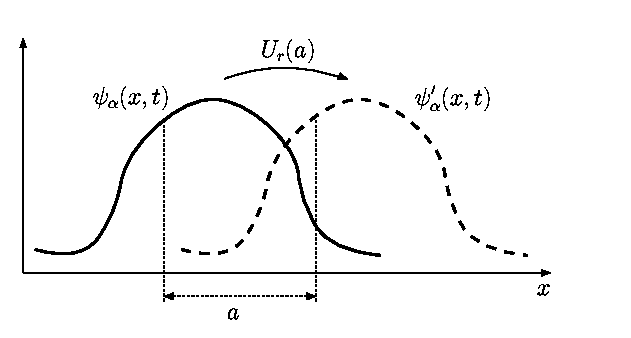
\includegraphics{pics/qmtranslacija.eps}}

Tražimo $U_{r}(a)$ takav da je
\begin{displaymath}
  \psi'_{\alpha}(x,t)= U_{r}(a)\psi_{\alpha}(x,t) \;.
\end{displaymath}
Imamo (iz crteža):
\begin{gather}
 \psi'_{\alpha}(x,t)=\psi_{\alpha}(x-a,t) \\
 \psi_{\alpha}(x-a,t)=U_{r}(a)\psi_{\alpha}(x,t) \qquad \text{(transf. je
  aktivna)} \label{optrans}
\end{gather}

Lijevu stranu jednadžbe razvijemo u Taylorov red i zbrojimo:
\begin{equation*}
\begin{split}
 \psi_{\alpha}(x-a,t)&=\psi_{\alpha}(x,t)-a\frac{\pd\psi_{\alpha}(x,t)}
{\pd x}+\frac{a^2}{2!}\frac{\pd^2 \psi_{\alpha}(x,t)}{\pd x^2}-\ldots \\
&=\left(1-a\frac{\pd}{\pd x}+\frac{a^2}{2!}\frac{\pd^2}{\pd x^2} - \ldots\right)
\psi_{\alpha}(x,t) \\
&=e^{-a \pd / \pd  x} \psi_{\alpha}(x,t)
\end{split}
\end{equation*}
Usporedbom vidimo da je operator translacije u 1D:
\begin{displaymath}
U_r(a)= e^{-a \pd / \pd  x}
\end{displaymath}
odnosno, u 3D,
\begin{displaymath}
U_r(\vec{a})= e^{-\vec{a}\cdot\nabla}
\end{displaymath}
Poznavajući kvantnomehaničku korespondenciju $-i\hbar\nabla \leftrightarrow
\vec{p}$ imamo konačno
\begin{equation}
U_r(\vec{a})= e^{-(i/\hbar)\vec{a}\cdot\vec{p}} \;.
\end{equation}
($e^{-\vec{a}\cdot\nabla}$ je operator translacije u koordinatnoj
reprezentaciji, a $e^{-(i/\hbar)\vec{a}\cdot\vec{p}}$ vrijedi u svakoj 
reprezentaciji.)

% Operatori translacije tvore troparametarsku Abelovu Lievu grupu
% $(\mathbb{R}^3, +)$ s generatorima $p_x, p_y, p_z$. Algebra:
% \begin{displaymath}
%   [p_i, p_j] = 0 \;, \qquad i,j = 1,2,3
% \end{displaymath}
% 
% Prije smo generatore definirali kao $X$ u relaciji $M=e^{\epsilon X}\in G$,
% a sada ekstrahiramo faktor $-i/h$ kako bismo imali izravnu korespondenciju
% između generatora grupe i odgovarajuće fizikalne veličine.
 
\subsection{Prostorne translacije - Blochov teorem$^*$}

\emph{Kristal} je sustav atoma koji je invarijantan na translacije 
za bilo koji vektor oblika:
\begin{equation}
  \vec{t}_{\vec{n}} \equiv n_1 \vec{a}_1 + n_2 \vec{a}_2 
  + n_3  \vec{a}_3 \qquad n_{1,2,3}\in\mathbb{Z}\;,
\label{tn}
\end{equation}
gdje su $\vec{a}_{1,2,3}$ tzv. \emph{primitivni vektori} koji definiraju
jediničnu čeliju kristalne rešetke. Prilikom izračuna valne funkcije 
elektronskog
oblaka u kristalu pogodno je zahtijevati da ona zadovoljava tzv.
\emph{Born-von Karmanove periodičke rubne uvjete}:
\begin{equation}
 \psi(\vec{r}) = \psi(\vec{r} + N_1 \vec{a}_1)= \psi(\vec{r} + N_2 \vec{a}_2)
= \psi(\vec{r} + N_3 \vec{a}_3) \;,
\end{equation}
gdje su $N_{1,2,3}$ neki fiksni vrlo veliki ($N_{1,2,3}\gg 1$) prirodni 
brojevi\footnote{
Ovakav zahtjev zamišlja topologiju kristala kao hiper-torusa, što je
dovoljno realistično jer nas ionako topologija ili površinska svojstva
kristala ovdje ne zanimaju, već samo svojstva ``bulk'' materijala poput
specifičnog toplinskog kapaciteta ili električne vodljivosti.
(Specifični toplinski kapacitet bakra je isti bez obzira da li je riječ
o ravnoj žici, petlji, ploči ili pak torusu.)}.

To dalje znači da operatori translacije zadovoljavaju
\begin{equation}
       U_{r}(N_j \vec{a}_j) = U_{r}(0) = 1 \qquad  j=1,2,3
\end{equation}
i odgovarajuća translacijska grupa simetrija ima $N\equiv N_1 N_2 N_3$
elemenata. Kako translacije komutiraju ova grupa je Abelova što
znači da ima $N$ ireducibilnih reprezentacija koje su
sve jednodimenzionalne (cf. npr. Zadatak 3.2).
Elementi grupe su generirani translacijom za primitivne vektore
$U_{r}(\vec{a}_j)$  pa tako imamo
\begin{equation}
U_{r}(\vec{a}_1)^{N_1} = 1 
\end{equation}
\begin{equation}
U_{r}(\vec{a}_1) = \exp\Big\{-2\pi i\: \frac{p_1 }{N_1}\Big\} \qquad 
 p_1 \in \{0,1,2,\ldots ,N_1 -1\} \;,
\end{equation}
tj. translacija za $\vec{a}_1$ može biti reprezentirana s
$N_1$ različitih operatora.  Općenita translacija za vektor 
$\vec{t}_{\vec{n}}$ (\ref{tn}) može onda biti reprezentirana jednodimenzionalnim
operatorima oblika
\begin{align}
 U_{r}(\vec{t}_{\vec{n}}) &=
 U_{r}(n_1 \vec{a}_1 + n_2 \vec{a}_2 + n_3  \vec{a}_3) \\
 &= U_{r}(\vec{a}_1)^{n_1} U_{r}(\vec{a}_2)^{n_2} U_{r}(\vec{a}_3)^{n_3} \\
 &= \exp\Big\{ -2\pi i \Big( \frac{n_1 p_1}{N_1} + \frac{n_2 p_2}{N_2} 
 + \frac{n_3 p_3}{N_3} \Big)\Big\} \;,
\label{blochirreps}
\end{align}
tj. s $N$ različitih operatora kako i očekujemo za grupu s $N$ IRREPsa.
Svaka od tih IRREPsa se onda može označiti s trojkom brojeva $(p_1, p_2, p_3)$
gdje svaki od brojeva $p_j$ može poprimiti bilo koju vrijednost iz
skupa $\{0, 1, 2, \ldots ,N_j -1\}$.
Operator translacije $U_{r}(\vec{t}_{\vec{n}})$ je u konkretnom IRREPsu 
 $(p_1, p_2, p_3)$ reprezentiran operatorom/brojem (\ref{blochirreps}).

Umjesto trojke $(p_1, p_2, p_3)$ za označavanje IRREPsa se obično
upotrebljavaju vektori $\vec{k}$ definirani na slijedeći način. Prvo
definiramo tzv. vektore \emph{recipročne rešetke} $\vec{b}_1, \vec{b}_2,
\vec{b}_3$ putem zahtjeva:
\begin{equation}
   \vec{a}_i\cdot \vec{b}_j = 2 \pi \delta_{ij} \qquad i,j = 1, 2, 3 \;.
\label{defb}
\end{equation}
Sada vektor $\vec{k}$ koji odgovara IRREPsu
$(p_1, p_2, p_3)$ definiramo kao
\begin{equation}
  \vec{k} \equiv \frac{p_1}{N_1}\vec{b}_1 + \frac{p_2}{N_2}\vec{b}_2 + 
  \frac{p_3}{N_3}\vec{b}_3 \;.
\label{defk}
\end{equation}
Iz (\ref{defk}), (\ref{defb}) i (\ref{blochirreps}) slijedi da je
operator translacije za $\vec{t}_{\vec{n}}$ u IRREPsu $\vec{k}$
dan s
\begin{equation}
 U_{r}^{(\vec{k})} (\vec{t}_{\vec{n}}) = 
 e^{-i \vec{k}\cdot \vec{t}_{\vec{n}}} \;,
\end{equation}
i odsad $N$ različitih $\vec{k}$-ova (\ref{defk}) labelira IRREPse.
Vidimo da dimenzija $\vec{k}$ odgovara valnom broju, tj. impulsu
podijeljenom s Planckovom konstantom.

Djelovanje ovih operatora translacije na valne funkcije u datom
IRREPsu mora biti kao i kod svih operatora translacije (\ref{optrans})
\begin{equation}
 e^{-i \vec{k}\cdot \vec{t}_{\vec{n}}} \psi_{\vec{k}}(\vec{r}) =
\psi_{\vec{k}}(\vec{r} - \vec{t}_{\vec{n}}) \;.
\label{bloch}
\end{equation}
Kako je riječ o običnim brojevima (a ne recimo diferencijalnim
operatorima) dobili smo razmjerno jednostavan uvjet koje valne funkcije
u kristalu moraju zadovoljavati da bi bile svojstvene funkcije operatora
translacije. Takve funkcije se nazivaju \emph{Blochove funkcije}, a
$\vec{k}$ je Blochov valni vektor.
Zašto su one zanimljive?

Kao prvo, ako ih (bez gubitka općenitosti) zapišemo u obliku
\begin{equation}
 \psi_{\vec{k}}(\vec{r}) = e^{+i \vec{k}\cdot \vec{r}} u_{\vec{k}}(\vec{r})
\end{equation}
onda odmah iz (\ref{bloch}) dobijemo uvjet 
\begin{equation}
  u_{\vec{k}}(\vec{r}) = u_{\vec{k}}(\vec{r} - \vec{t}_{\vec{n}})  \;,
\end{equation}
dakle Blochove funkcije su oblika 
$e^{+i \vec{k}\cdot \vec{r}} u_{\vec{k}}(\vec{r})$,
gdje je $u_{\vec{k}}(\vec{r})$ periodička funkcija na rešetci. Isto,
\secret{Blochove funkcije su svojstvene funkcije operatora translacije na rešetci.?}

S druge strane, operator translacije na rešetci komutira s Hamiltonijanom
\begin{equation}
    [H, U_{r}^{(\vec{k})} (\vec{t}_{\vec{n}}) ] = 0 \;.
\end{equation}
Komutiranje s kinetičkim dijelom je trivijalno jer su i kinetički dio
hamiltonijana i operator translacije funkcije samo impulsa. 
Komutiranje s potencijalom
je posljedica periodičnosti $V(\vec{r}) = V(\vec{r}-\vec{t}_{\vec{n}})$.
(Pokažite ovo! \secret{$U_{r}^{\dagger}(\vec{t}_{\vec{n}})
A(\vec{r}) U_{r}(\vec{t}_{\vec{n}}) = A(\vec{r}-\vec{t}_{\vec{n}})$
za svaki operator $A(\vec{r})$, pa onda tvrdnja slijedi za $A=V$.})
Posljedica komutiranja dvaju operatora je da oni imaju zajedničke
svojstvene funkcije. To onda povlači

\textbf{Blochov teorem}: Valne funkcije periodičke rešetke mogu se
izabrati kao Blochove funkcije.

Ovo onda olakšava rješavanje Schr\"{o}dingerove jednadžbe
za rešetku jer je potrebno naći samo funkcije $u_{\vec{k}}(\vec{r})$ za
svaki $\vec{k}$,
a njihova periodičnost umnogome pojednostavljuje taj zadatak.
Vidi fiziku čvrstog stanja za primjere. U fizici čvstog stanja se
također obično izvodi Blochov teorem. Ovdje je naglasak dan
na grupno-teorijski pristup tj. korespondenciju s reprezentacijama
grupe translacija.


\subsection{Vremenske translacije$^*$}

Slično kao kod prostorne imamo
\begin{displaymath}
 \psi'_{\alpha}(x,t) = \psi_{\alpha}(x,t-\tau) = U_{t}(\tau)\psi_{\alpha}(x,t)
\end{displaymath}
I opet Taylorovim razvojem
\begin{equation*}
\begin{split}
 \psi_{\alpha}(x,t-\tau)&=\psi_{\alpha}(x,t)-\tau\frac{\pd\psi_{\alpha}(x,t)}
{\pd t}+\ldots \\
&=e^{-\tau \pd / \pd  t} \psi_{\alpha}(x,t)
\end{split}
\end{equation*}
Sada korespondencijom $i\hbar\pd /\pd t \leftrightarrow H$
imamo
\begin{displaymath}
U_t(\tau)= e^{(i/h)H\tau} \;,
\end{displaymath}
ali ovo vrijedi samo za $H$ konstantan u vremenu (kakav on jest u većini
nama zanimljivih slučajeva). Za diskusiju vidi Sakurai, sect. 2.1.

\paragraph{Vremenska evolucija}
Vremenska translacija daje sustav koji ima isto ponašanje u vremenskom
trenutku $t+\tau$ kao originalni sustav u trenutku $t$. Vremenska
\emph{evolucija} nekog sustava se isto može dobiti iz ovog gore, ako
primijetimo da je
\begin{displaymath}
\psi_{\alpha}(x,t-\tau)=e^{(i/h)H\tau}\psi_{\alpha}(x,t)
\end{displaymath}
pa zamjenom $\tau\equiv t-t'$ imamo 
\begin{displaymath}
\psi_{\alpha}(x,t')=e^{-(i/h)H(t'-t)}\psi_{\alpha}(x,t)
\end{displaymath}

Vrijedi dakle
\begin{displaymath}
U_{\text{evolucija}}(t' -t)=U^{-1}_{\text{translacija}}(t' -t)
=U_{\text{translacija}}(t -t') \;.
\end{displaymath}


\paragraph{Očuvane veličine} 
Promotrimo operator $A$ takav da je
$[H,A]=0$. Neka je $\psi(x,t)$ svojstveno stanje od $A$ tj.
\[
  A\psi(x,t) = a \psi(x,t)
\]
Tada to isto stanje nakon vremena $(t'-t)$ zadovoljava
\[
  A\psi(x,t')= A e^{-(i/h)H(t'-t)} \psi(x,t) =
 e^{-(i/h)H(t'-t)} A \psi(x,t) = a \psi(x,t')
\]
tj. $A$ je očuvana veličina. Npr. za slobodnu česticu $H=p^2/2m$ 
$\imp$ 
\[
   [H,p]=\frac{1}{2m}[p^2,p]=0
\]
i impuls je očuvan.

Veličine koje komutiraju s Hamiltonijanom su očuvane u vremenu.

\subsection{Rotacije}

\centerline{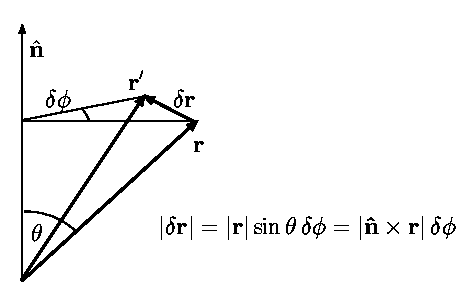
\includegraphics[scale=0.8]{pics/infrotacija.eps}}
Infinitezimalna rotacija je (vidi sliku):
  \begin{displaymath}
  \vec{r}\to\vec{r}'=\vec{r}+\delta\phi\, \unitn\times\vec{r}  \;.
 \end{displaymath}
To znači da, po analogiji s translacijama, valna funkcija zarotiranog
sustava treba zadovoljavati

\begin{equation*}
\begin{split}
\psi_{\alpha}'(\vec{r}, t)&=\psi_{\alpha}(R(\hat{\vec{n}},\delta \phi)^{-1}
\vec{r}, t) \\
 &=\psi_{\alpha}(\vec{r}-\delta\phi\hat{\vec{n}}\times\vec{r}, t) \\
 &=\psi_{\alpha}(\vec{r}, t)-(\delta\phi\hat{\vec{n}}\times\vec{r})\cdot
  \nabla\psi_{\alpha}(\vec{r}, t) \\
 &= \psi_{\alpha}(\vec{r}, t)-\frac{i}{\hbar}(\delta\phi\hat{\vec{n}}\times
  \vec{r})\cdot \vec{p}\psi_{\alpha}(\vec{r}, t) \\
 &= \left(1-\frac{i}{\hbar}\vec{L}\cdot\hat{\vec{n}}\delta\phi \right)
  \psi_{\alpha}(\vec{r}, t)
\end{split}
\end{equation*}

Rotaciju za konačni kut dobijemo kompozicijom N rotacija za $\delta\phi / N$
gdje $N\to\infty$:

\begin{equation}
\mathcal{D}(\hat{\vec{n}}, \phi)=\lim_{N\to\infty}
\left(1-\frac{i}{\hbar}\vec{L}\cdot\hat{\vec{n}}\delta\phi \right)^N
= e^{-(i/\hbar)\vec{L}\cdot\hat{\vec{n}}\phi}
\end{equation}

Izotropija prostora povlači očuvanje momenta impulsa: $[H,L_{i}]=0$.

Operatori $L_i$, $i=x,y,z$ zadovoljavaju komutacijske relacije
\begin{equation}
   [L_x, L_y] = i\hbar  L_z  \qquad \text{i ciklične zamjene}
\end{equation}
%(Vidi vježbe za izvod ovog i definiciju $\epsilon_{ijk}$.)

\section{Spin$^*$}

Klasična fizika $\to$ različita transformacijska svojstva pri
rotacijama $\to$ \emph{tenzori}.

Kakva je situacija u kvantnoj mehanici?

Promotrimo rotaciju vektora valnih funkcija:

\begin{displaymath}
  \vec{\Psi}(\vec{r},t) \equiv (\psi_{x}(\vec{r}, t),
 \psi_{y}(\vec{r}, t), \psi_{z}(\vec{r}, t))
\end{displaymath}

Ovakav vektor će nam biti zanimljiv npr. pri razmatranju čestice koja se vrti 
oko svoje osi i kod koje nas ne zanima samo 
njen položaj u prostoru već i njena orijentacija.

Kao i ranije, tražimo operator s djelovanjem
\begin{displaymath}
  \vec{\Psi}'(\vec{r},t) = \mathcal{D}
(\vec{\hat{n}},\phi) \vec{\psi}(\vec{r},t) \;,
\end{displaymath}
gdje je $\vec{\Psi}'(\vec{r},t)$ valna funkcija zarotiranog sustava.

\centerline{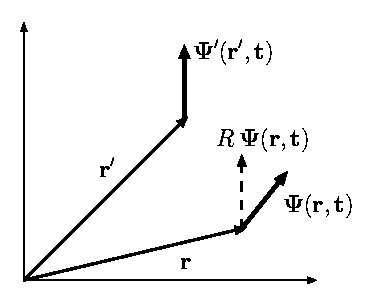
\includegraphics{pics/spin.eps}}

Iz slike vidimo:
\begin{gather*}
\vec{\Psi}'(\vec{r}',t)=R \vec{\Psi}(\vec{r},t) \\
\vec{\Psi}'(\vec{r},t)=R \vec{\Psi}(R^{-1}\vec{r},t) 
\end{gather*}
pa imamo, slično kao kod rotacije jednokomponentne funkcije:
\begin{equation*}
\begin{split}
\mathcal{D}(\vec{\hat{n}},\delta\phi)\vec{\Psi}(\vec{r}, t)&=
 R \vec{\Psi}(R(\hat{\vec{n}},\delta \phi)^{-1}
\vec{r}, t) \\
 &=\vec{\Psi}(R(\hat{\vec{n}}, \delta\phi)^{-1}\vec{r}, t)+
\delta\phi \hat{\vec{n}}\times\vec{\Psi}(
R(\hat{\vec{n}}, \delta\phi)^{-1}\vec{r},t) \\
 &=\vec{\Psi}(\vec{r}-\delta\phi\hat{\vec{n}}\times\vec{r}, t)+
\delta\phi \hat{\vec{n}}\times\vec{\Psi}(\vec{r},t) + O(\delta\phi^2) \\
 &= \vec{\Psi}(\vec{r}, t)-\frac{i}{\hbar}(\delta\phi\hat{\vec{n}}\cdot
  \vec{L})\vec{\Psi}(\vec{r}, t)+
\delta\phi \hat{\vec{n}}\times\vec{\Psi}(\vec{r},t) + O(\delta\phi^2)
\end{split}
\end{equation*}
Imamo dodatni član $\delta\phi \hat{\vec{n}}\times\vec{\Psi}(\vec{r},t)$
kojeg ćemo drugačije napisati pomoću tripleta matrica definiranih na
slijedeći način:
\begin{displaymath}
(S_j)_{ik} = i\hbar\epsilon_{ijk} \quad j=1,2,3 \;.
\end{displaymath}
Konkretno
\begin{align}
S_1& =i\hbar
\begin{pmatrix}
0 & 0 & 0 \\
0 & 0 &-1 \\
0 & 1 & 0
\end{pmatrix} = i\hbar X_1 \\
S_2& = i\hbar
\begin{pmatrix}
0 & 0 & 1 \\
0 & 0 & 0 \\
-1 & 0 & 0
\end{pmatrix} = i\hbar X_2 \\
S_3& = i\hbar
\begin{pmatrix}
0 & -1 & 0 \\
1 & 0 & 0\\
0 & 0 & 0
\end{pmatrix} = i\hbar X_3 
\end{align}
Uz tako definirane matrice imamo
\begin{displaymath}
\begin{split}
[\hat{\vec{n}}\times\vec{\Psi}]_i &=
\epsilon_{ijk}\hat{n}_j\Psi_k \\
&= -\frac{i}{\hbar}\hat{n}_j (S_j)_{ik}\Psi_k\\
&= -\frac{i}{\hbar}(\hat{\vec{n}}\cdot\vec{S})_{ik}\Psi_k \;,
\end{split}
\end{displaymath}
što znači
\begin{equation*}
\mathcal{D}(\vec{\hat{n}},\phi)\vec{\Psi}(\vec{r}, t)=
 \left(1-\frac{i}{\hbar}(\vec{L}+\vec{S})\cdot\hat{\vec{n}}\delta\phi \right)
  \Psi(\vec{r}, t)
\end{equation*}
odnosno, za konačne rotacije:
\begin{equation}
\mathcal{D}(\hat{\vec{n}}, \phi)=
 e^{-(i/\hbar)(\vec{L}+\vec{S})\cdot\hat{\vec{n}}\phi}
\end{equation}

Matrice $S_i$ također zadovoljavaju komutacijske relacije angularnog
momenta.

\secret{.... (Adjungirane REP  --- strukturne konstante) ...}

$\vec{S}$ - intrinsični angularni moment (spin)

$\vec{J}=\vec{L}+\vec{S}$  - ukupni angularni moment

Za izolirani sustav $[H, \vec{J}] = 0$, ali moguće je da je
$[H, \vec{L}] \neq 0$, $[H, \vec{S}] \neq 0$, npr. pri vezanju spina
i orbite u atomu. (Elektron usljed orbitiranja ``vidi'' magnetsko polje
jezgre koje interagira s njegovim magnetskim momentom.)

Vidimo da se trokomponentna valna funkcija transformira drugačije
od jednokomponentne. Koje su još mogućnosti? Treba nam općenita teorija
reprezentacija grupe rotacija u kvantnoj mehanici.

\subsection*{Zadaci}

\begin{enumerate}[label=\arabic{chapter}.\arabic*.]

\item Pokažite da je operator translacije kvantnomehaničkog stanja,
 $U_{r}(\vec{a}) = \exp \{-\frac{i}{\hbar} \vec{p}\cdot \vec{a} \}$
unitaran. Razmotrite situaciju u koordinatnoj reprezentaciji gdje
je $\vec{p} = -i \hbar \nabla$. Zašto ovaj $i$ ne kvari unitarnost?

\item Neka $\psi(\vec{r}, t)$ zadovoljava Schr\"{o}dingerovu jednadžbu.
Pokažite da će prostorno translatirana $\psi(\vec{r}, t)' = 
U_{r}(\vec{a}) \psi(\vec{r}, t)$ također zadovoljavati Schr\"{o}dingerovu
jednadžbu ako i samo ako je $[H, \vec{p}] = 0$

\item Koristeći fundamentalne kvantnomehaničke komutatore
\begin{displaymath}
 [x_i, p_j] = i\hbar \delta_{ij}\;, \qquad
 [x_i, x_j] = [p_i, p_j] = 0 \;,
\end{displaymath}
te svojstva Levi-Civita tenzora, izračunajte komutacijske
relacije angularnog momenta $[L_i, L_j]$.

\item Pokažite da operatori spina $S_i$ također zadovoljavaju komutacijske
relacije angularnog momenta.

\item Pokažite da je $[\vec{J}^2, J_i] = 0$.
\end{enumerate}
